\documentclass[10pt]{beamer}

\usetheme[progressbar=frametitle]{metropolis}
\usepackage{appendixnumberbeamer}

\usepackage{booktabs}
\usepackage[scale=2]{ccicons}
\usepackage{fontawesome}
\usepackage{pgfplots}
\usepgfplotslibrary{dateplot}
\usepackage{mathtools}
\usepackage{xspace}
\newcommand{\themename}{\textbf{\textsc{metropolis}}\xspace}
%\usepackage{caption}
%\usepackage{hyperref}
%\usepackage[citestyle=authoryear,natbib=true,backend=bibtex]{biblatex}
%\usepackage{biblatex}
%\bibliography{rl}
%\usepackage{natbib}

\title{A Brief Survey of Reinforcement Learning}
\subtitle{A modern beamer theme}
\date{\today}
% \date{11 Dec 2018}
\author{Giancarlo Frison}
%\institute{ \faTwitter gfrison}
% \titlegraphic{\hfill\includegraphics[height=1.5cm]{logo.pdf}}
\begin{document}

\setbeamertemplate{frame footer}{\faTwitter gfrison 2018}

\maketitle

\begin{frame}{Table of contents}
  \setbeamertemplate{section in toc}[sections numbered]
  \tableofcontents[hideallsubsections]
\end{frame}

\section{Introduction}
\begin{frame}[fragile]{What is Reinforcement Learning}
	\begin{figure}[t!]	
	\centering
	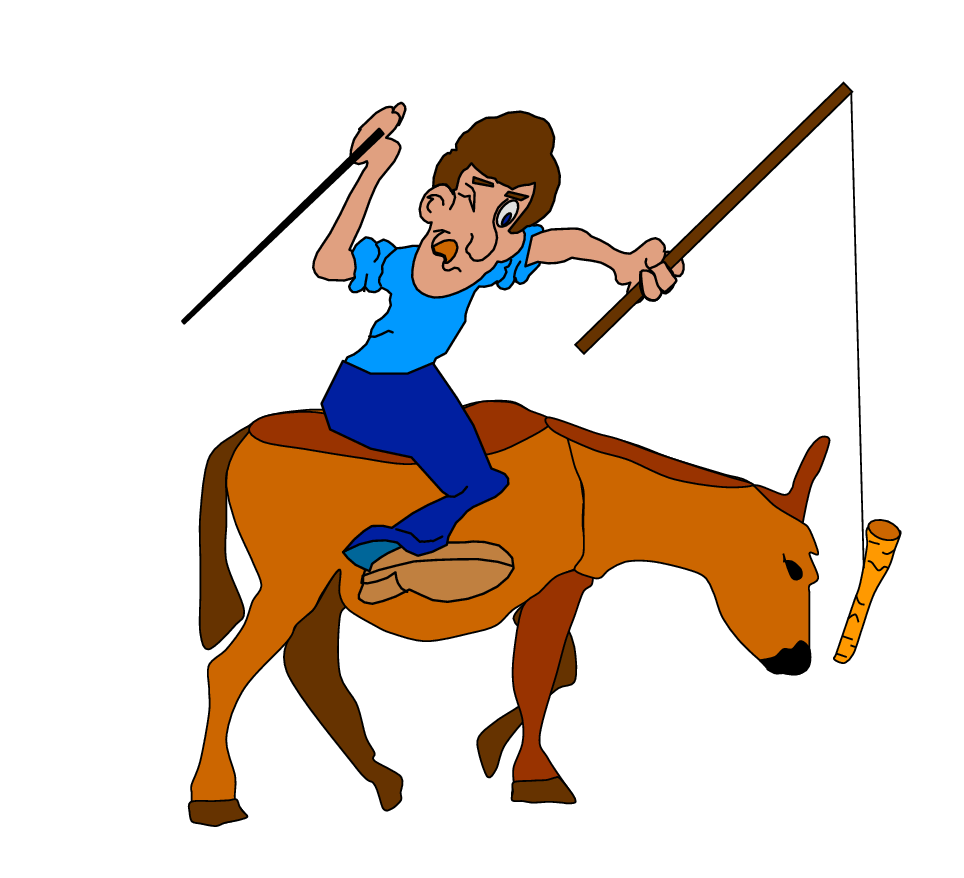
\includegraphics[scale=0.3]{img/donkey.png}
	\cite{donkey}
	\end{figure}
	\textsc{Reinforcement learning} is an area of machine learning concerned with how software agents ought to take actions in an environment so as to maximize some notion of cumulative reward.
\end{frame}

\begin{frame}[fragile]{What it is Not}
Although RL can induce to an optimization, there are major differences within:
  \begin{itemize}[<+- | alert@+>]
    \item \alert<4>{Supervised learning}
	\item Mathematical optimization
	\item Genetic programming
  \end{itemize}
\end{frame}

\begin{frame}[fragile]{Metropolis}

    

  The \themename theme is a Beamer theme with minimal visual noise
  inspired by the \href{https://github.com/hsrmbeamertheme/hsrmbeamertheme}{\textsc{hsrm} Beamer
  Theme} by Benjamin Weiss.

  Enable the theme by loading

  \begin{verbatim}    \documentclass{beamer}
    \usetheme{metropolis}\end{verbatim}

  Note, that you have to have Mozilla's \emph{Fira Sans} font and XeTeX
  installed to enjoy this wonderful typography.
\end{frame}
\begin{frame}[fragile]{Sections}
  Sections group slides of the same topic

  \begin{verbatim}    \section{Elements}\end{verbatim}

  for which \themename provides a nice progress indicator \ldots
\end{frame}
\section{Multi-armed Bandit}
\begin{frame}{Multi-armed Bandit}
	\begin{figure}[t!]	
	\centering
	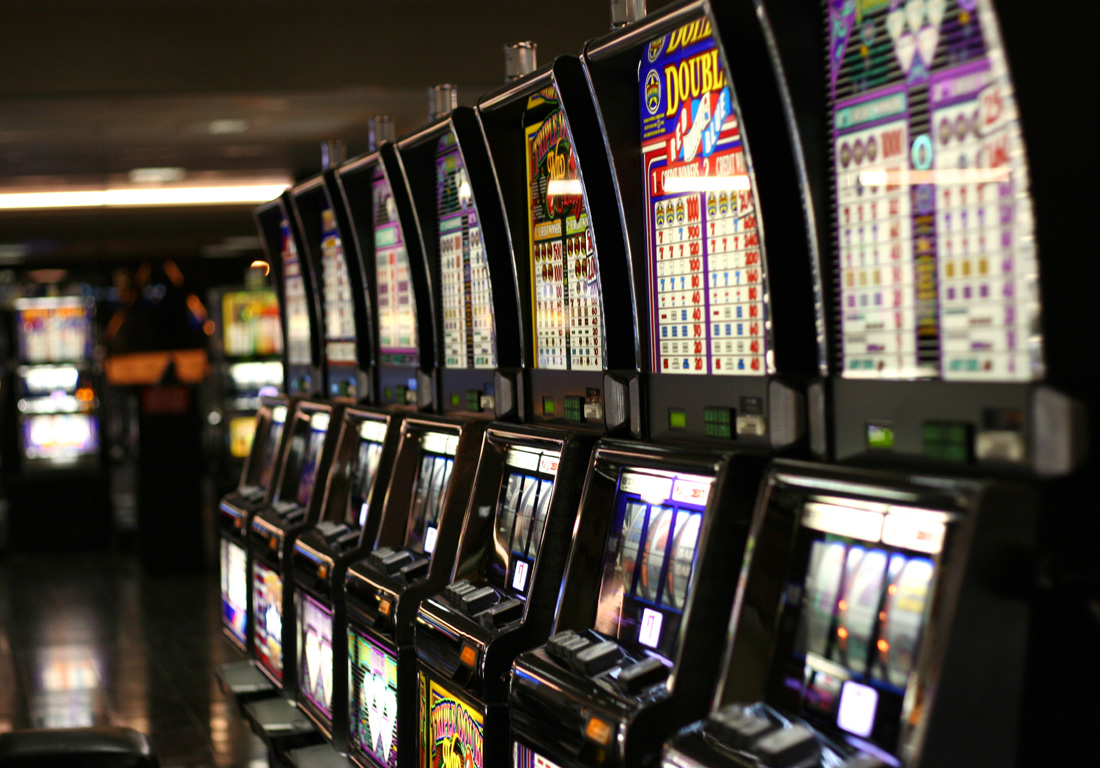
\includegraphics[scale=0.2]{img/Las_Vegas_slot_machines.jpg}
	\end{figure}
	The multi-armed bandit problem has been the subject of decades of intense study in statistics, operations research, electrical engineering, computer science, and economics \cite{bandit}
\end{frame}

\begin{frame}
	\frametitle{\begin{math} Q \end{math} Value's Action}
	\begin{figure}[t!]
		\centering
		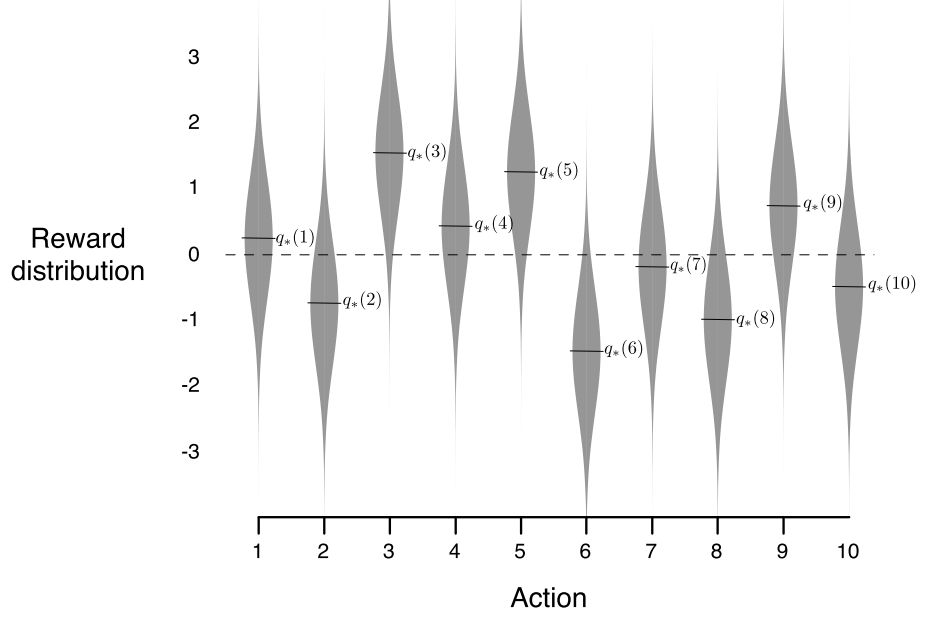
\includegraphics[scale=0.25]{img/bandit-reward-dist.png}
	\end{figure}
	An example bandit problem \cite{Montague1999}. Obtained measures after repeated pullings with 10 arms.
\end{frame}

\begin{frame}
	\frametitle{\begin{math} Q \end{math} Value's Action}
	\begin{math} \mathbf{Q_n} \end{math} is the estimated value of its action after $ n $ selections.	
	$$ Q_{n+1} = \frac{R_1 +R_2 + ... +R_{n}}{n} $$
	A more scalable formula, updates the average with incremental and small constant:
	$$ Q_{n+1} = Q_n + \frac{1}{n}(R_n-Q_n)$$
	General expression of the badint algorithm at the fundation of RL. \begin{math}Target\end{math} could be considered the reward $ R $ by now.
	$$ \mathbf{NewEstimate = OldEstimate + StepSize(Target-OldEstimate)}$$
\end{frame}

\begin{frame}
\frametitle{Gambler's Dilemma}
When pulled, an arm produces a random payout drawn independently of the past. Because the distribution of payouts corresponding to each arm is not listed, the player can learn it only by experimenting.
	\begin{columns}
		\begin{column}{0.5\textwidth}
			\begin{alertblock}{Exploitation}
		Earn more money by exploiting arms that yielded high payouts in the past.
			\end{alertblock}
		\end{column}
		\begin{column}{0.5\textwidth}  %%<--- here
			\begin{alertblock}{Exploration}
		Exploring alternative arms may return higher payouts in the future.
			\end{alertblock}
		\end{column}
	\end{columns}
\end{frame}

\section{Markov Decision Process}
\begin{frame}
	\frametitle{Definition of MDP}
	\begin{figure}
		\includegraphics[scale=0.15]{img/2015_DARPA_Robotics_Challenge_150606-N-PO203-090.jpg}	
		\caption{2015 DARPA Robotics Challange \cite{mdp-robot}}
	\end{figure}
	Despite as in bandits, MDP formalizes the decision making (Policy $\pi$) in sequential steps, aggregated in Episodes. 
\end{frame}

\begin{frame}
	\frametitle{Actions and States}
	\begin{figure}
	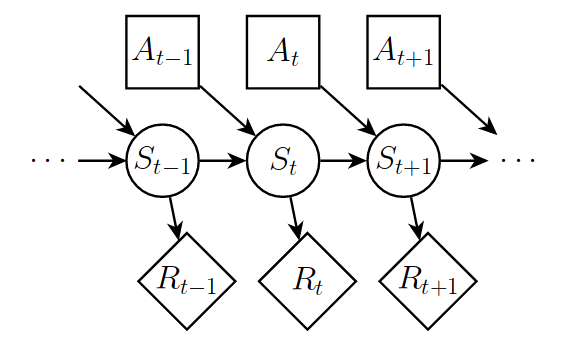
\includegraphics[scale=0.2]{img/mdp-states.png}
	\caption{Model representation of MDP \cite{mdp-process}}
	\end{figure}
	MDP strives to find the best $\pi$ to all possible states. 
	In Markov processes, the selected action depends \textbf{only} on current state.
\end{frame}

\begin{frame}
	\frametitle{How to evaluate an Agent?}
	Given that:
	\begin{itemize}
		\item Agent maximizes future rewards.
		\item $\pmb{\gamma}$ is the rewards' discount factor. 
		\item Policy $\pmb{\pi}$ defines a particular way of acting.
		\item $\mathbf{v_π(s)}$ is the expected return from $\mathbf{s}$ following $\pmb{\pi}$ \emph{thereafter}.
		\item $\mathbf{q_π(s, a)}$ is the $\mathbf{v_π(s)}$ taking action $\mathbf{a}$
	\end{itemize}
	
	A recursive algorithm could be indentified, known as the \textsc{Bellman equation}. Iteratevely computes the value $\mathbf{Q}$ from the terminal state:
	$$ \mathbf{Q_t(s, a) = R_{t + 1} + \gamma max[v(S_{t+1})]} $$

	
		
\end{frame}

\begin{frame}
	\frametitle{Grid World}
	\begin{columns}
		\begin{column}{0.5\textwidth}
			\begin{tikzpicture}[scale=2]
			\draw[step=0.5cm,color=gray] (-1,-1) grid (1,1);
			\node at (-0.75,+0.75) { \faFlagCheckered };
			\node at (-0.25,+0.75) {-1};
			\node at (+0.25,+0.75) {-1};
			\node at (+0.75,+0.75) {-1};
			\node at (-0.75,+0.25) {-1};
			\node at (-0.25,+0.25) {-1};
			\node at (+0.25,+0.25) {-1};
			\node at (+0.75,+0.25) {-1};
			\node at (-0.75,-0.25) {-1};
			\node at (-0.25,-0.25) {-1};
			\node at (+0.25,-0.25) {-1};
			\node at (+0.75,-0.25) {-1};

			\node at (-0.75,-0.75) {-1};
			\node at (-0.25,-0.75) {-1};
			\node at (+0.25,-0.75) {-1};
			\node at (+0.75,-0.75) { \faFlagCheckered  };
			\end{tikzpicture}
		\end{column}
		\begin{column}{0.5\textwidth} 
			\begin{itemize}
				\item $ A = {up, down, right, left}$
				\item Terminal states are the flagged boxes.		
				\item $R_t = 0$ for terminal states.
				\item $R_t = -1$ for other states.
			\end{itemize}			 
		\end{column}
	\end{columns}
	The problem is to define the best $\pmb{\pi}$. Value function is computed by iterative policy evaluation. 
\end{frame}

\begin{frame}
	\frametitle{Grid World}
	\begin{columns}
		\begin{column}{0.1\textwidth}
		\end{column}
		\begin{column}{0.2\textwidth}
			\textbf{Iteration}
		\end{column}
		\begin{column}{0.3\textwidth}
			\textbf{Calculated $V_k$}
		\end{column}
		\begin{column}{0.3\textwidth} 
			\textbf{Policy $\pi_k$}
		\end{column}
		\begin{column}{0.1\textwidth}
		\end{column}
	\end{columns}
	\vfill
	\begin{columns}
		\begin{column}{0.1\textwidth}
		\end{column}
		\begin{column}{0.2\textwidth}
			k = 1
		\end{column}
		\begin{column}{0.3\textwidth}
			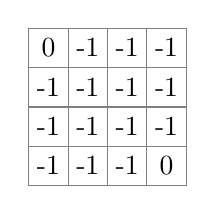
\begin{tikzpicture}[scale=1]
			\draw[step=0.5cm,color=gray] (-1,-1) grid (1,1);
			\node at (-0.75,+0.75) { 0 };
			\node at (-0.25,+0.75) {-1};
			\node at (+0.25,+0.75) {-1};
			\node at (+0.75,+0.75) {-1};
			\node at (-0.75,+0.25) {-1};
			\node at (-0.25,+0.25) {-1};
			\node at (+0.25,+0.25) {-1};
			\node at (+0.75,+0.25) {-1};
			\node at (-0.75,-0.25) {-1};
			\node at (-0.25,-0.25) {-1};
			\node at (+0.25,-0.25) {-1};
			\node at (+0.75,-0.25) {-1};

			\node at (-0.75,-0.75) {-1};
			\node at (-0.25,-0.75) {-1};
			\node at (+0.25,-0.75) {-1};
			\node at (+0.75,-0.75) { 0  };
			\end{tikzpicture}
		\end{column}
		\begin{column}{0.3\textwidth} 
			\begin{tikzpicture}[scale=1]
			\draw[step=0.5cm,color=gray] (-1,-1) grid (1,1);
			\node at (-0.75,+0.75) { \faFlagCheckered };
			\node at (-0.25,+0.75) { $\leftarrow$ };
			\node at (+0.25,+0.75) {?};
			\node at (+0.75,+0.75) {?};
			\node at (-0.75,+0.25) {$\uparrow$};
			\node at (-0.25,+0.25) {?};
			\node at (+0.25,+0.25) {?};
			\node at (+0.75,+0.25) {?};
			\node at (-0.75,-0.25) {?};
			\node at (-0.25,-0.25) {?};
			\node at (+0.25,-0.25) {?};
			\node at (+0.75,-0.25) {$\downarrow$};

			\node at (-0.75,-0.75) {?};
			\node at (-0.25,-0.75) {?};
			\node at (+0.25,-0.75) {$\rightarrow$};
			\node at (+0.75,-0.75) { \faFlagCheckered  };
			\end{tikzpicture}
		\end{column}
		\begin{column}{0.1\textwidth}
		\end{column}
	\end{columns}
	\vfill
	\begin{columns}
		\begin{column}{0.1\textwidth}
		\end{column}
		\begin{column}{0.2\textwidth}
			k = 1
		\end{column}
		\begin{column}{0.3\textwidth}
			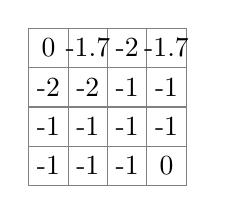
\begin{tikzpicture}[scale=1]
			\draw[step=0.5cm,color=gray] (-1,-1) grid (1,1);
			\node at (-0.75,+0.75) { 0 };
			\node at (-0.25,+0.75) {-1.7};
			\node at (+0.25,+0.75) {-2};
			\node at (+0.75,+0.75) {-1.7};
			\node at (-0.75,+0.25) {-2};
			\node at (-0.25,+0.25) {-2};
			\node at (+0.25,+0.25) {-1};
			\node at (+0.75,+0.25) {-1};
			\node at (-0.75,-0.25) {-1};
			\node at (-0.25,-0.25) {-1};
			\node at (+0.25,-0.25) {-1};
			\node at (+0.75,-0.25) {-1};

			\node at (-0.75,-0.75) {-1};
			\node at (-0.25,-0.75) {-1};
			\node at (+0.25,-0.75) {-1};
			\node at (+0.75,-0.75) { 0  };
			\end{tikzpicture}
		\end{column}
		\begin{column}{0.3\textwidth} 
			\begin{tikzpicture}[scale=1]
			\draw[step=0.5cm,color=gray] (-1,-1) grid (1,1);
			\node at (-0.75,+0.75) { \faFlagCheckered };
			\node at (-0.25,+0.75) { $\leftarrow$ };
			\node at (+0.25,+0.75) {?};
			\node at (+0.75,+0.75) {?};
			\node at (-0.75,+0.25) {$\uparrow$};
			\node at (-0.25,+0.25) {

			};
			\node at (+0.25,+0.25) {?};
			\node at (+0.75,+0.25) {?};
			\node at (-0.75,-0.25) {?};
			\node at (-0.25,-0.25) {?};
			\node at (+0.25,-0.25) {?};
			\node at (+0.75,-0.25) {$\downarrow$};

			\node at (-0.75,-0.75) {?};
			\node at (-0.25,-0.75) {?};
			\node at (+0.25,-0.75) {$\rightarrow$};
			\node at (+0.75,-0.75) { \faFlagCheckered  };
			\end{tikzpicture}
		\end{column}
		\begin{column}{0.1\textwidth}
		\end{column}
	\end{columns}
\end{frame}

\section{Titleformats}


\begin{frame}{Metropolis titleformats}
	\themename supports 4 different titleformats:
	\begin{itemize}
		\item Regular
		\item \textsc{Smallcaps}
		\item \textsc{allsmallcaps}
		\item ALLCAPS
	\end{itemize}
	They can either be set at once for every title type or individually.
\end{frame}

{
    \metroset{titleformat frame=smallcaps}
\begin{frame}{Small caps}
	This frame uses the \texttt{smallcaps} titleformat.

	\begin{alertblock}{Potential Problems}
		Be aware, that not every font supports small caps. If for example you typeset your presentation with pdfTeX and the Computer Modern Sans Serif font, every text in smallcaps will be typeset with the Computer Modern Serif font instead.
	\end{alertblock}
\end{frame}
}
\begin{frame}[allowframebreaks]{References}

  \bibliography{rl}
  \bibliographystyle{abbrv}

\end{frame}

\begin{frame}[allowframebreaks]{List of Figures}
    \listoffigures
\end{frame}

\end{document}
